\documentclass{article}
\usepackage{graphicx}
\usepackage{graphics}
\graphicspath{{/home/user/images/},{/home/personnels/berhe/TextClassification/}}
\usepackage{amsmath}
\usepackage{fancyhdr}

\setlength{\parindent}{0em}
\setlength{\parskip}{1em}
\renewcommand{\baselinestretch}{1.5}

\pagestyle{fancy}
\fancyhf{}
\rfoot{Page \thepage}
\lfoot{text classification}

\title{Text Classification }
\author{Aman Berhe}

\begin{document}
\maketitle
\newpage
\section{Visualizations}
the following figures show the visualization of both Pompe diseases and Amytrophic Lateral 
Diseases for 60 articles each
\subsection{Amytrophic Lateral Disease}
The data collected has been preprocessed.the "<unknown>" lemma has been replaced by the word 
and also the different punctuation symbols has also been removed since they do not make any sense.

The Dimention of the Positive and negative words: 
\begin{table}[h!]
  \centering
  \caption{Amytrophic Lateral Disease Dimension}
  \label{tab:table1}
  \begin{tabular}{l|c|r}
      & positive & negative\\
    \hline
      Words &  2295  & 9774 \\
    \hline
      vector &  1:only lemmas  & 1:only lemmas \\
  \end{tabular}
\end{table}
\begin{table}[h!]
  \centering
  \caption{Pompe Disease Dimension}
  \label{tab:table1}
  \begin{tabular}{l|c|r}
      & positive & negative\\
    \hline
      Words &  3291  & 9247 \\
    \hline
      vector &  1:only lemmas  & 1:only lemmas \\
  \end{tabular}
\end{table}
\newpage
Here is the Item Frequency of the words$($Items$)$

positive 

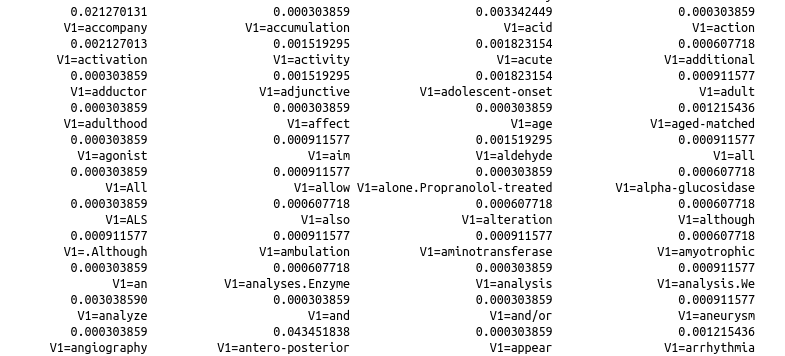
\includegraphics[width=0.8\linewidth]{freqPosit.png}\\
negative

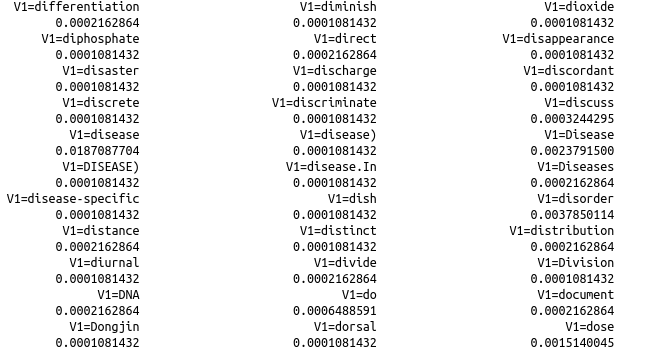
\includegraphics[width=0.8\linewidth]{freqneg.png}\\
The Histogram of the words and their frequencies\\
	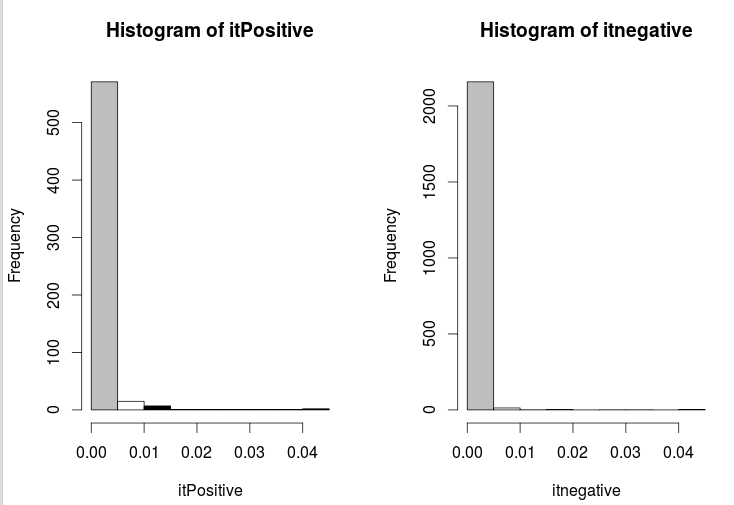
\includegraphics[width=0.8\linewidth]{Amytrophic1.png}\\
	
	ItemFrequency Plot Showing the words along the histogram
	
	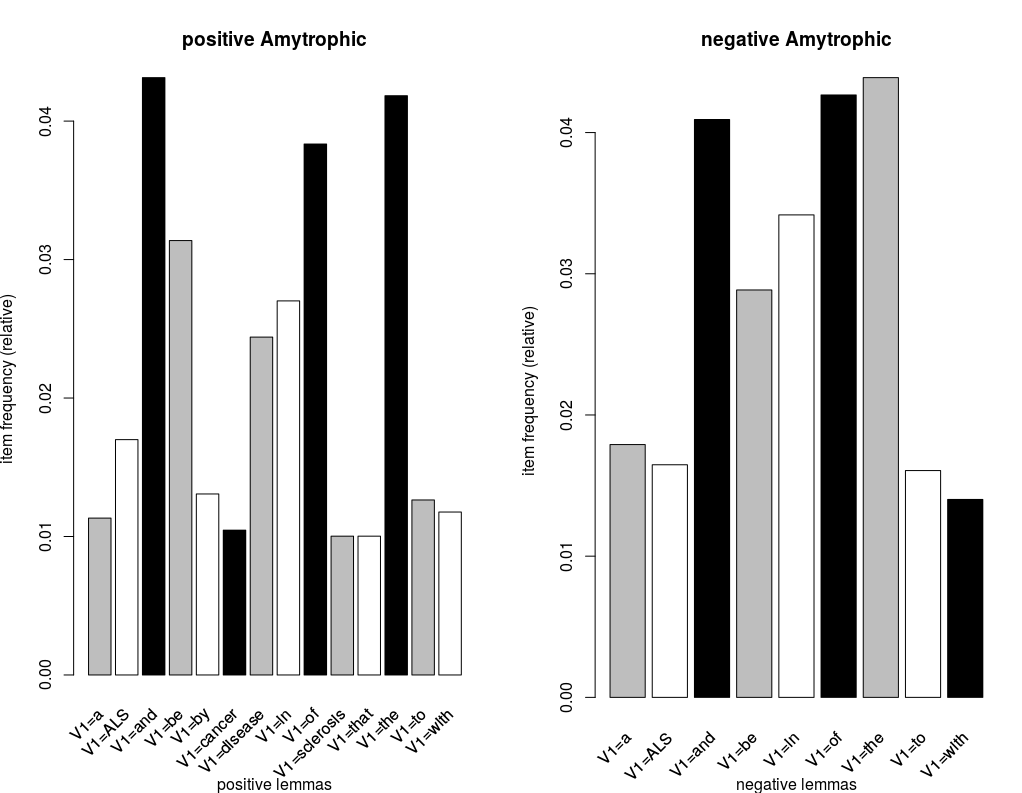
\includegraphics[width=0.8\linewidth]{Amytrophic2.png}\\
	on the positive words the 'and' word is most frequent and in the negative the 'the' is more frequent
	
	this figure shows the combination of the two, as where they occur
	
	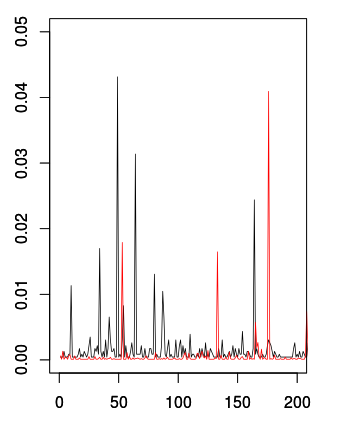
\includegraphics[width=0.8\linewidth]{Amytrophic3.png}\\
	the following figure shows some example of the words and their number of occurrence for the positive words 
	
	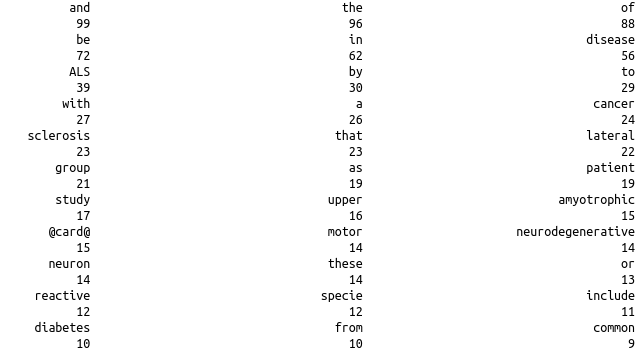
\includegraphics[width=0.8\linewidth]{Amytrophic4.png}\\
	The following two images shows the number of occurrence and number of words that occupy that amount of frequency which is the same as the zipf's law
	
	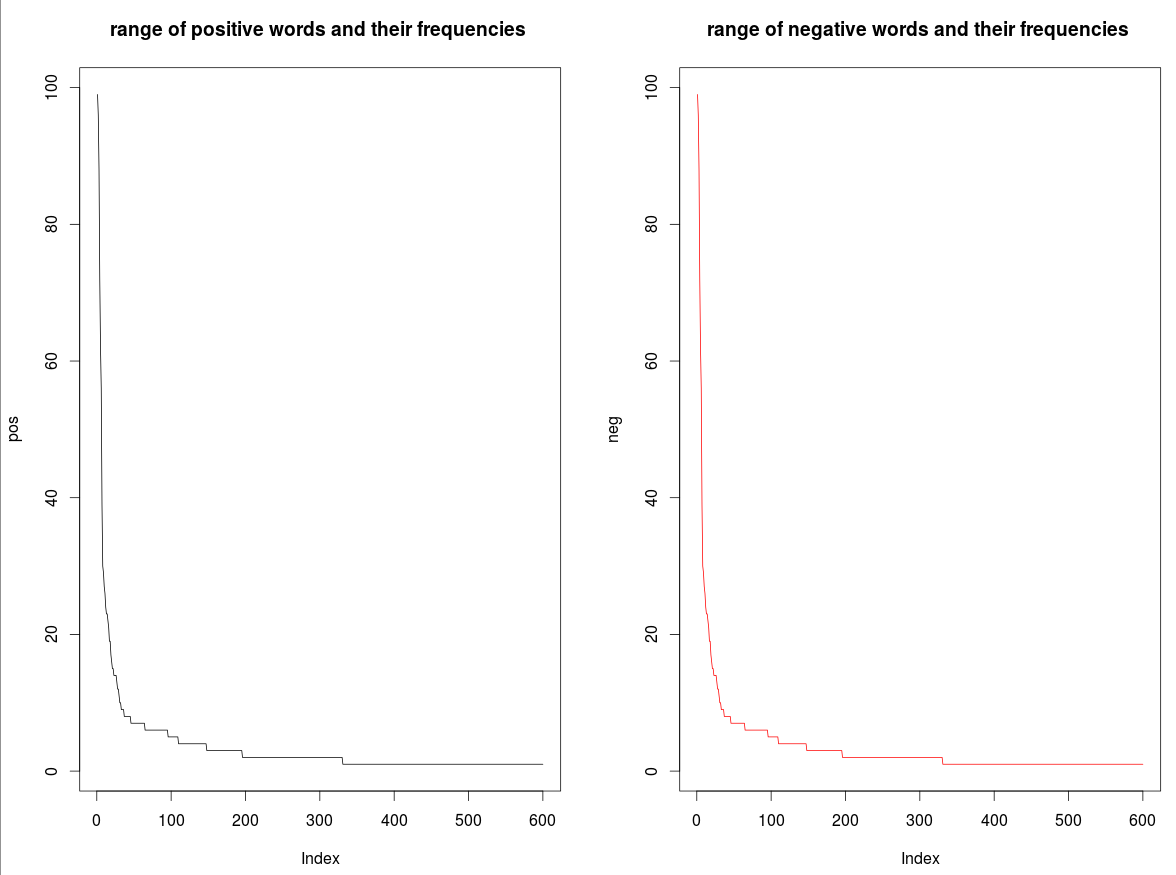
\includegraphics[width=0.8\linewidth]{Amytrophic5.png}\\
	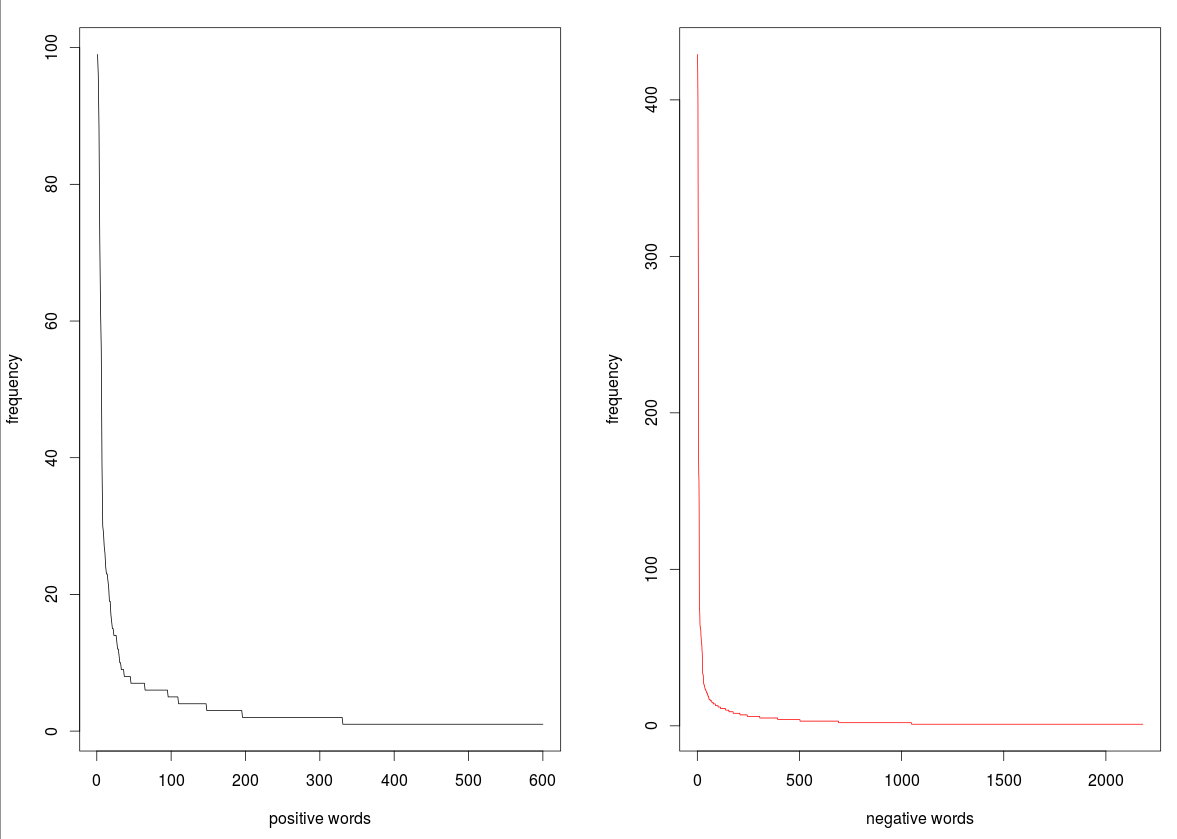
\includegraphics[width=0.8\linewidth]{Amytrophic6.png}\\
	\newpage
	the following figure shows the Zipf's law on the histogram of top 20 words according to their occurrence
	
	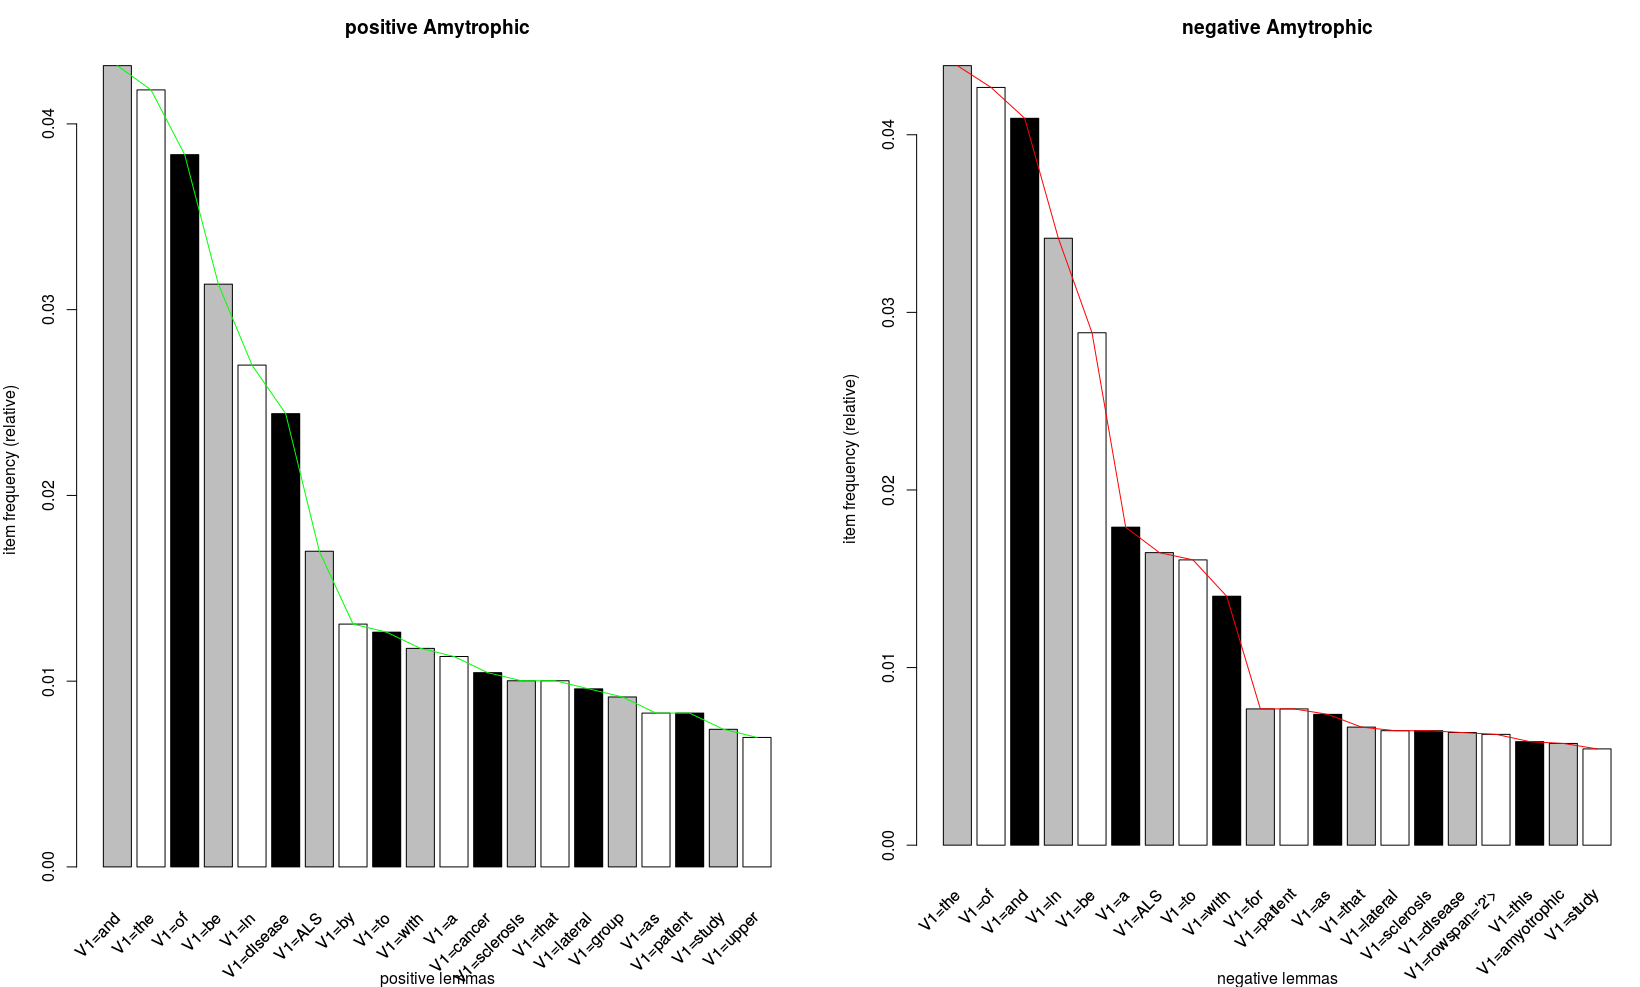
\includegraphics[width=0.8\linewidth]{Amytrophic7.png}\\
	
	Gross Rate has been computed using the number of occurrence and total number of words. Here are the Graphs
	
	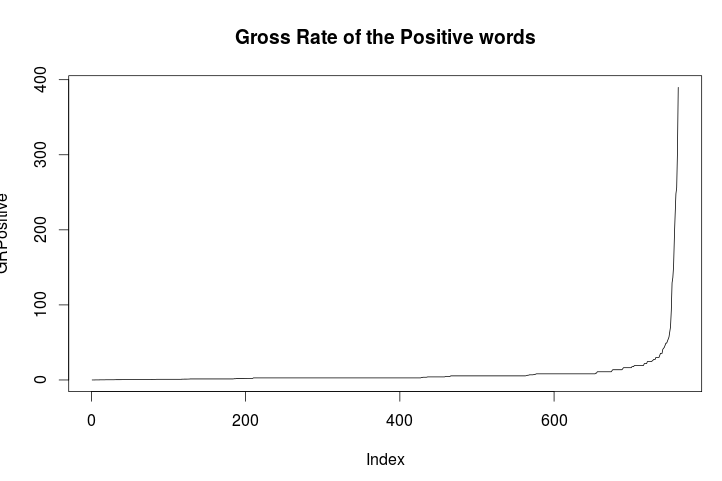
\includegraphics[width=0.8\linewidth]{GRpos.png}\\
	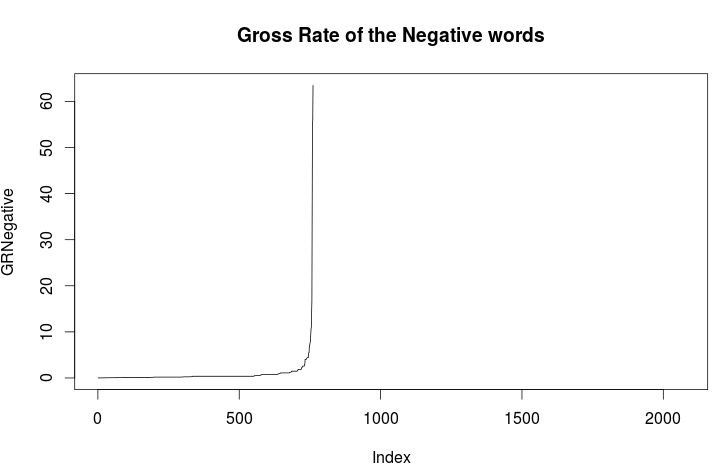
\includegraphics[width=0.8\linewidth]{GRneg.png}\\
\section{Accepting Sentence}
using the prompt I accept a sentence to be classified then I lemmatize it. 
E.eg

classify$<$-readSentence()

Enter your sentence: 

Enzyme replacement therapy (ERT) is important for the treatment of lysosomal storage disorders. Hypersensitivity reactions with ERT have been reported, and in these cases, desensitisation with the enzyme is necessary. Here we report the cases of 3 patients with lysosomal storage disorders, including Pompe disease and mucopolysaccharidosis type I and VI, who had IgE-mediated hypersensitivity reactions and positive skin tests. Successful desensitisation protocols with the culprit enzyme solution were used for these patients. All 3 patients were able to safely receive ERT with the desensitisation protocol.

$>$cassifyTagged$<$-taggedText(classify)

The out put looks like this

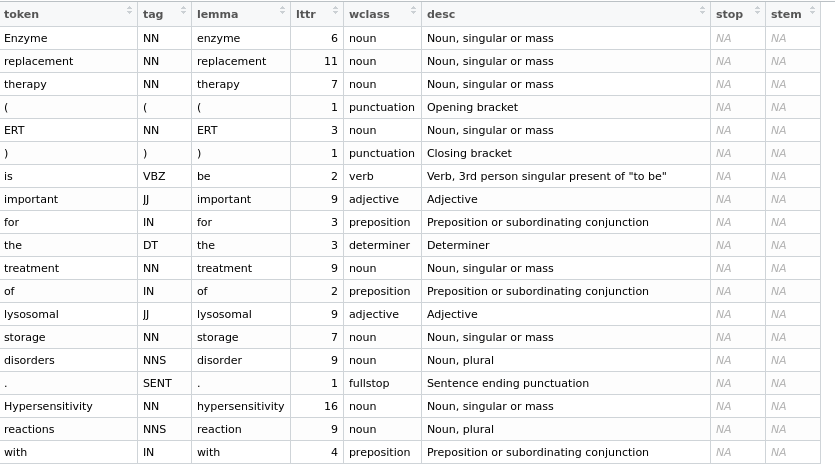
\includegraphics[width=0.8\linewidth]{Korpus1.png}\\
here is the Graph

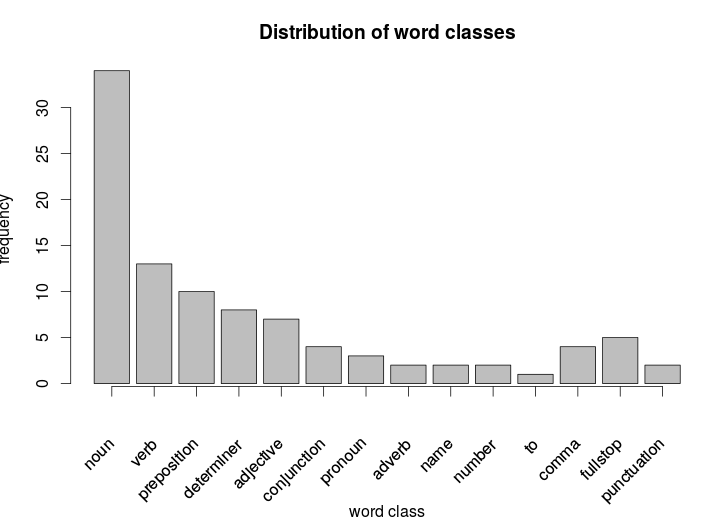
\includegraphics[width=0.8\linewidth]{korpus2.png}

\end{document}